
\onecolumn %% updated on 2017.7.19

\begin{center}
\hrule
\vspace{10pt}
{\bigsf KAGRA OBSERVATORY}
\label{kagra}
\vspace{10pt}
\hrule
\end{center}

\begin{multicols}{2}
KAGRA observatory is located in the Ikenoyama-mountain on the border
between Gifu and Toyama prefecture, about 35 km south of Toyama city in
Japan. The observatory was established in 2016 in order to operate Large
-scale Cryogenic Gravitational Wave Telescope (nicknamed “KAGRA”). KAGRA
itself has a L-shape tunnel facility, and it is located more than 200m
under Mt.Ikeno-yama. The corner station of the L-shape tunnel is
accessible through a 500-m horizontal access tunnel from Atotsu area.
The observatory has its own surface research buildings and rental space
in the community center of Hida city located about 5km away from the
Atotsu entrance of KAGRA.

KAGRA aims to observe several gravitational waves (GWs) per a year with
its designed sensitivity as one of observatories of the world GW
detection network including Advanced-LIGO, Advanced-Virgo and planned
LIGO-India. KAGRA project (formerly named LCGT) was partially approved
in 2010 as one of Leading-edge Research Infrastructure Program, and also
supported by Program for Promoting Large-scale Science Projects, Subsidy
for Facilities Expense and Grants-in-Aid for Scientific Research from
Ministry of Education, Culture, Sports, Science and Technology (MEXT).

In KAGRA project, Institute for Cosmic Ray Research plays a role of a
host promoting institute, and National Astronomical Observatory in Japan
(NAOJ) and High Energy Accelerator Research Organization (KEK) are the
main support organizations, then more than 297 researchers in 85
institutes and universities in the world are collaborating for
construction and data analysis of KAGRA.

The tunnel excavation started in May 2012, and finished in March 2014.
After that, the basic laboratory environment was prepared until
September 2015. A Michelson interferometer with 3km arm (iKAGRA) was
demonstrated in March 2016, and the first engineering run was performed
until May 2016.  At present (April 2019), all the interferometer components had been installed to complete 
the KAGRA Observatory that adopts a power recycled Fabry-Perot Michelson type interferometer 
with the resonant sideband extraction and the interferometer is under commissioning.
We plan to start the joint observation with LIGO and Virgo within 2019.

\end{multicols} 

\medskip
\medskip
\medskip

\begin{figure}[htbp]
\begin{minipage}{0.5\textwidth}
\begin{center}
%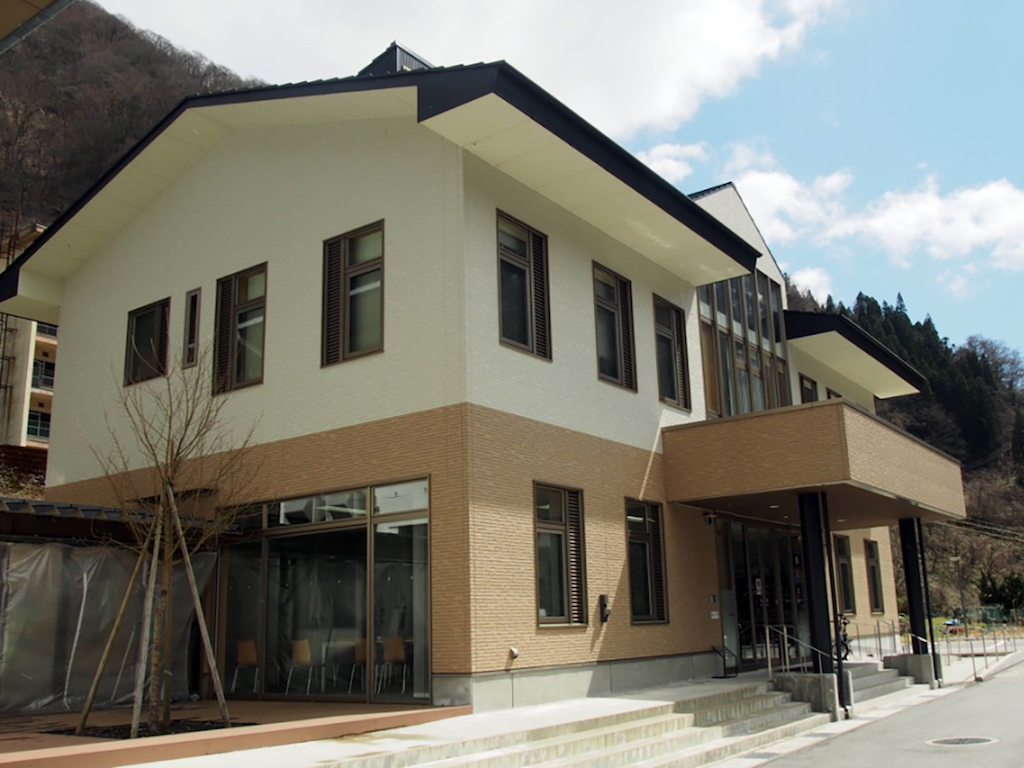
\includegraphics[width=0.8\textwidth]{./obs/kagra/building.jpg}
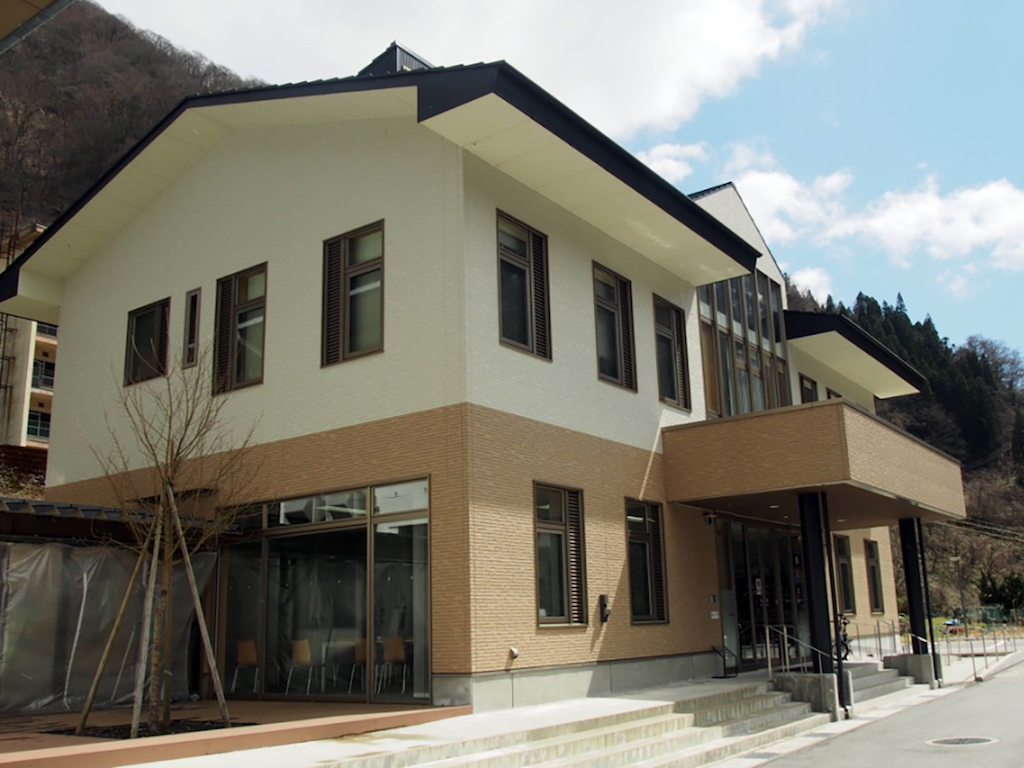
\includegraphics[height=6cm, bb=0 0 1024 768]{./obs/kagra/building.jpg}
\caption{Surface Research Building.}
\end{center}
\end{minipage}
%
\begin{minipage}{0.5\textwidth}
\begin{center}
%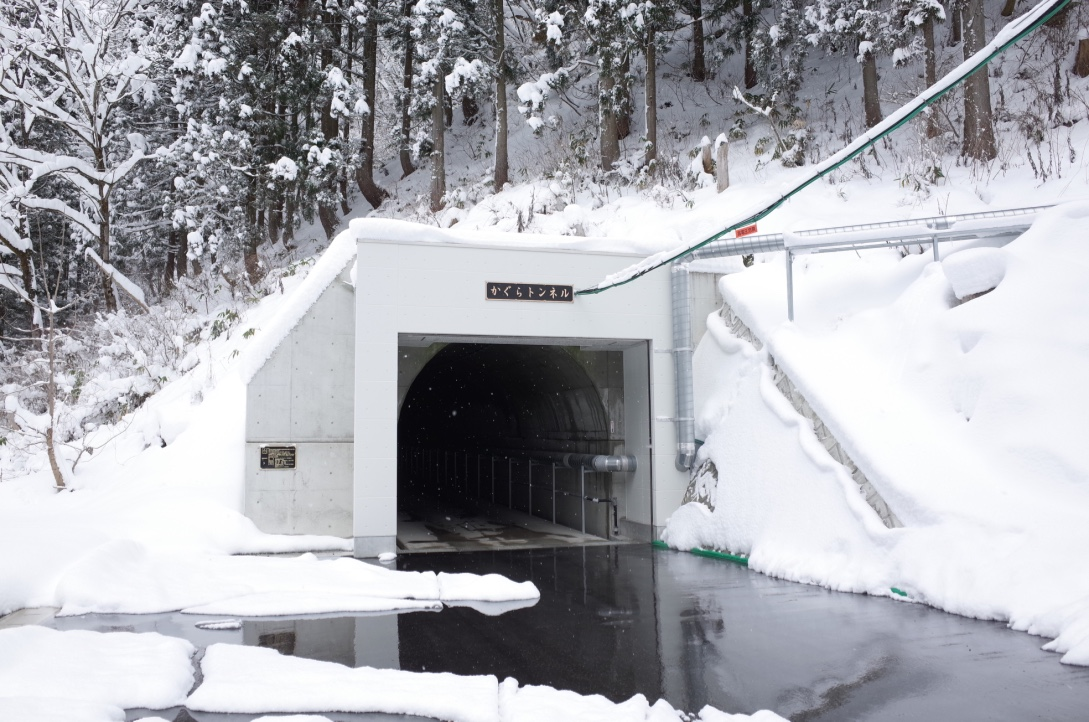
\includegraphics[width=0.8\textwidth]{./obs/kagra/entrance.jpg}
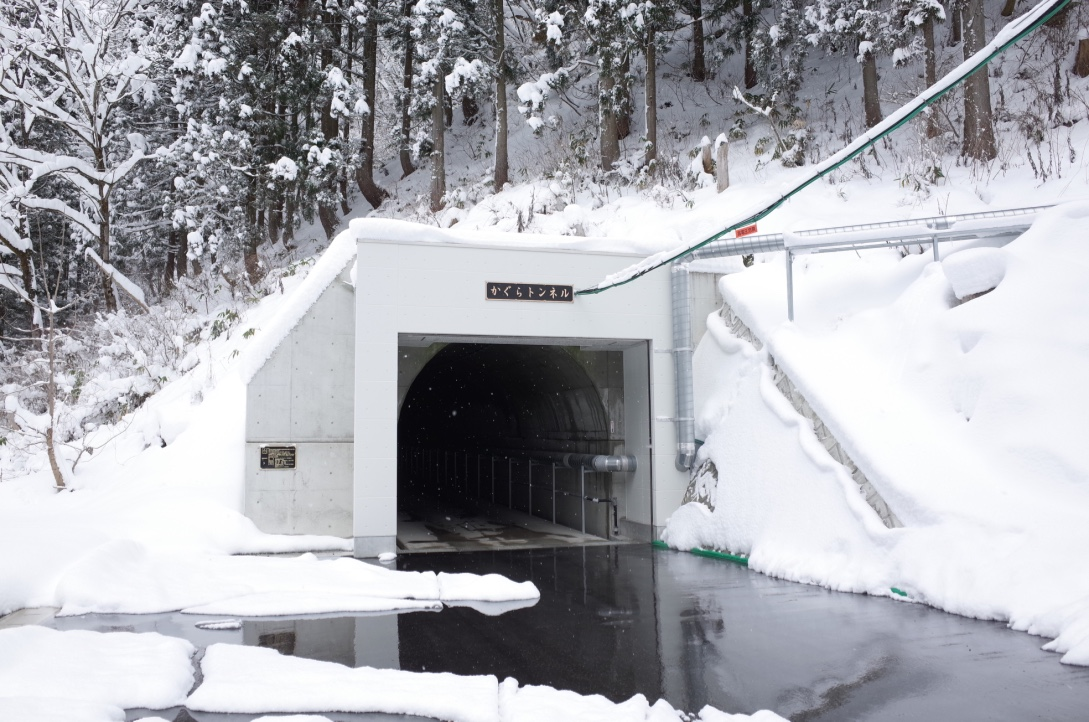
\includegraphics[height=6cm, bb=0 0 1089 722]{./obs/kagra/entrance.jpg}
\caption {Atotsu Entrance of KAGRA.}
\end{center}
\end{minipage}
\end{figure}


